\documentclass[12pt, fleqn]{article}
\usepackage{../../../template/template}

%сам документ
\begin{document}
\begin{center}
  \huge Практика по дифференциальным уравнениям, 3 сем

  \Large (преподаватель Звягинцева Т. Е.)

  \large Записал Костин П.А.
\end{center}

Данный документ неидеальный, прошу сообщать о найденных недочетах в \href{https://vk.com/drab_existence_a}{вконтакте}
\tableofcontents
\newpage

%Замечания
\section{Введение}
Разрешимо в квадратурах=разрешимо в интеграллах\\
$y(x)$ - неизв. функция\\
$F(x,y,y',y'',...,y^{(n)})=0$\\
$y^{(n)}=f(x,y,...,y^{(n-1)})$\\
(1) $y'=f(x,y)$ - дифференциальное уравнение 1-го порядка

\begin{example}
    $y'=y$, решение $y=c e^x$
\end{example}

\begin{definition}
    Задача Коши: найти решение $y=\phi(x): \phi(x_0)=y_0$ ((2) $(x_0,y_0)$)
\end{definition}

Считаем, что $f(x,y) \in C(G)$\\
И пока что предполагаем, что $d f(x,y) \in C(G)$ (решение существует), $dy \in C(G)$ (решение единственное)\\
$(x_0,y_0) \in G$ $y=\phi(x)$ - решение (1) $\Ra \phi'(x_0)=f(x_0,y_0)$ $(y_0=\phi(x_0))$\\
В каждой точке области G определено направление касательной к кривой, проходящей через эту точку\\
\begin{definition}
    Кривые, в которых направление поля постоянно называются изоклины
\end{definition}

\begin{Example}[стоим изоклины]
    \[y'=\frac{y}{x}\]
    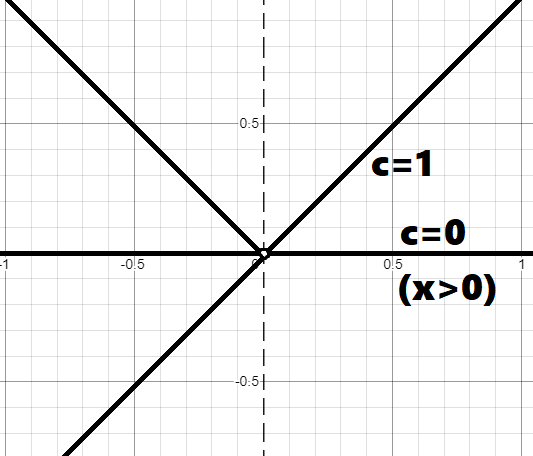
\includegraphics[scale=0.3]{pics/EasyIsoclines.png}\\
    \[x \neq 0,\q \frac{y}{x}=c(=tg \alpha)\text{ - уравнение изоклин}\]
    \[(y'=f(x,y) \Ra y'=c \Ra f(x,y)=c)\]
    \[\Ra y=cx\]
    \[\text{При } c=0\ (\ctg \alpha = 0 \Ra \alpha = 0) \Ra y=0\]
    \[\text{При } c=1\ (\ctg \alpha = 1 \Ra \alpha = \frac{\pi}{4}) \Ra y=x\]
    \[\text{З. Коши для (-1,1): }y=-x,\ x<0\]
\end{Example}

\begin{Example}[больше изоклин]
    \[y'=-\frac{y}{x} \Ra -\frac{y}{x}=c \text{ - уравнение изоклин}\]
    \[\Ra c=0\ (tg \alpha = 0)\Ra y=0\]
    \[\Ra c=1\ (\alpha = \frac{\pi}{4})\Ra y=-x\]
    \[\Ra c=\sqrt{3}\ (\alpha=\frac{\pi}{3})\Ra y=-\sqrt{3}x\]
\end{Example}

\begin{Example}[16, дополнительно] \ \\
    Написать уравнение геометрического места точек перегиба графиков решений уравнений:
    \[a)\q y'=y-x^2\]
    \[b)\q y'=f(x,y)\]
\end{Example}

\begin{sol}
    Условие перегиьа графика $y=f(x)$ - это $y''=0$\\
    a) $y'=y-x^2$
    \[y''=y'-2x=(y-x^2)-2x=0 \Ra y=x^2+2x\]
    b) Возьмем полный лифференциал от обеих частей равенства:
    \[d y'=d f(x,y) \Ra
    d y'=\dfrac{\d f}{\d x}d x+\dfrac{\d f}{\d y} d y
    \Ra \dfrac{d y'}{d x} = \dfrac{\d f}{\d x}+\dfrac{\d f d y}{\d y d x}\]
    \[\Ra y''=f'_x+f'_y y'=0 \Ra f'_x+f'_y y'=0\]
\end{sol}

\begin{Example}[замена переменной спасёт]
    \[y'=\sqrt{4x+2y-1}\]
\end{Example}
    \[\text{Пусть } z=4x+2y-1 \Ra z'=4+2y' \Ra \frac{z'-4}{2}=\sqrt{z}\]
    \[\frac{z'}{2}=\sqrt{z}+2 \Ra \frac{dz}{\sqrt{z}+2}=2dx\]
    (дорешать)

\begin{Example}[не пугаться замен]
    \[y'=\cos(y-x)\]
    \[y-x=z \Ra z'=y'-1\]
    \[z'=\cos z-1\]
    \[\frac{dz}{\cos z - 1}=dx\]
    \[\cos z=1\]
    \[z=2\pi k,\q k \in \Z\]
    \[y=x+2\pi k\]
\end{Example}

\begin{Example}[асимптота]
    \[y'=y^2-1,\q y \equiv 1,\ y \equiv -1\]
    \[y'>0 \lra y^2>1\]
    \[y'<0 \lra y^2<1\]
    \[y''=2y y'\]
    \[y''=2yy(y^2-1)\]
    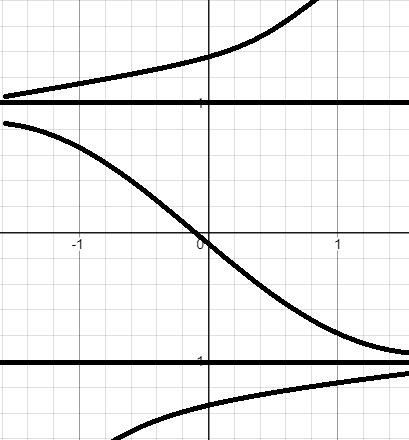
\includegraphics[scale=0.3]{pics/resh1.png}
\end{Example}

\begin{example}[теоретическая задача]
    Доказатать, что решение ограничено сверху или снизу\\
    \[Y'=P_n(y),\ n=2m-1,\ m \in \N\]
    У многочлена нечетной степени всегда есть вещественный корень, $y_j$ - корень, $j=1,...,k$, $y=y_j$ - реш. Значит остальные решения не пересекают на графике это $\Ra$ те котороые снизу, ограничены сверху, те которые сверху ограничены снизу\\
    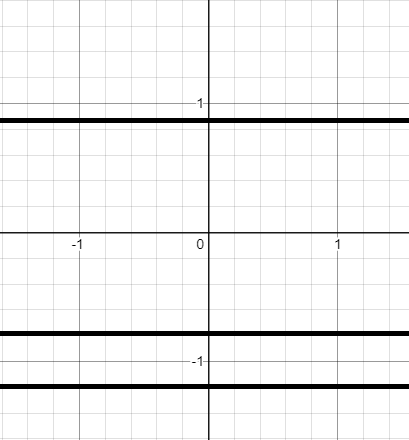
\includegraphics[scale=0.3]{pics/resh2.png}
\end{example}

\begin{example}[24, дополнительно]
  Составить диф. уравнение для семейства линий $y=a x^2 + b e^x$
  \[\Ra
  \begin{cases}
    y'=2a x + b e^x\\
    y'=2a + b e^x
  \end{cases}\]
  Нетрудно найти:
  \[a=\frac{y'-y''}{2(x-1)}\]
  Подставляя во второе уравнение:
  \[b=\frac{y'' x - y'}{e^x (x-1)}\]
  После подстановки в исходное:
  \[y'' x(x-2)-y'(x^2-2)+2(x-1)y=0\]
\end{example}

\section{Геометрические уравнения}

\begin{Example}
    \[y'=\frac{y}{x+y}\]
    \[y \neq x\]
    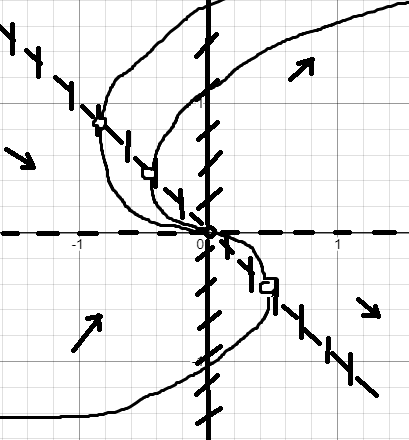
\includegraphics[scale=0.3]{pics/resh3.png}\\
    \[y \equiv 0\text{ - реш}\]
    \[y+x>0 \equiv y>-x\]
    \[y>0\]
    \[\frac{y}{z+y}=c \text{ - ур-ие изоклин}\]
    \[c=1 \q y=x+y\]
    \[y=cx+cy\]
    \[y(1-c)=cx\]
    \[y=\frac{c}{1-c}x,\q c \neq 1\]
    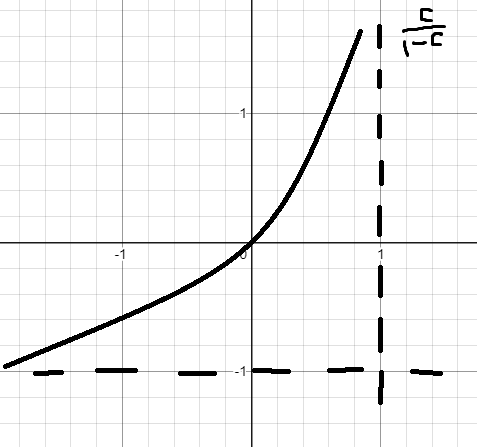
\includegraphics[scale=0.3]{pics/resh4.png}\\
    (упр.) Подставить точки
\end{Example}

\begin{example}
    \[y'=y-x^2 \Ra y=x^2+c\]
    Сократится тогда, когда уравнение второй степени $y=x^2+ax+b$, подставим: $2x+a=ax+b \Ra a=2 \ b=2$, значит $y=x^2+2x+2$ - решение\\
    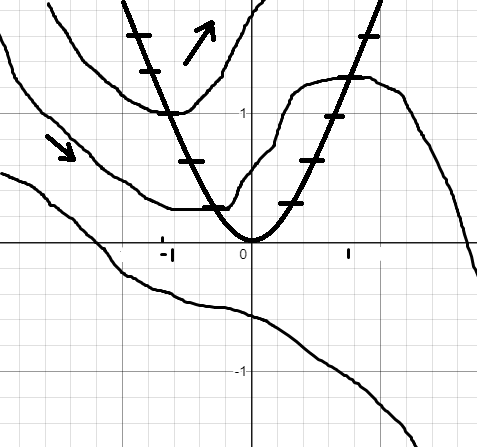
\includegraphics[scale=0.3]{pics/resh5.png}
    \[y''=y'-2x=y-x^2-2x,\q y=x^2+2x\]
\end{example}

\begin{example}\ \\
    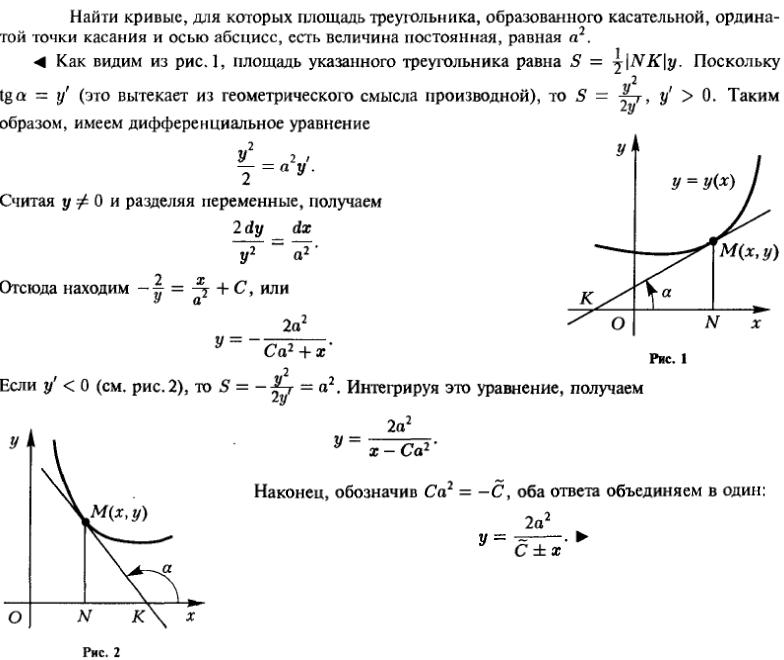
\includegraphics[scale=0.7]{pics/z71.jpg}
\end{example}

\section{Однородные уравнения}
\begin{definition}
    $M(x,y)$ - однор. ур-ие степени k, если $\forall \lambda>0 \q $ $M(\lambda x, \lambda y) = \lambda^k M(x,y)$
\end{definition}

\begin{definition}
    Уравнение $M(x,y) dx + N(x,y) dy=0$ - однородное, если $M,N$ - однородное одинаковой степени k
\end{definition}

\begin{definition}
    Уравнение $y'=f(x,y)$ - однородное, если $f(x,y)$ - однородное \\ степени 0
\end{definition}

\begin{example}[однородное уравнение]
    $x y'-y=x \tg \frac{y}{x}$\\
    $y'=\frac{y}{x}+\tg \frac{y}{x}$\\
    Замена $y=t x$\\
    То есть мы подставляем сперва $y=ay$, $x=ax$ и если a сокращаются, то уравнение однородное и можно сделать замену $y=tx$\\
    $y'=t' x+t$\\
    $dy=t dx+x dt$\\
    $t' x = \tg t$
\end{example}

Дз: 73, 76, 80, 84, 107, 109, 110, 101-112 (выбрать любую), 113

\begin{example}[пересекающиеся прямые]
    $(2x-4+6)dx+(x+y-3)dy=0$, чтобы сделать его однородным сделаем замену из системы (они не 0)\\
    $\begin{cases} 2x-4+6 = 0 \\ x+y-3=0 \end{cases} \Ra \begin{cases} x=\w{x}+1 \\ y=\w{y}+2 \end{cases}$\\
    $(2\w{x}-4\w{y})d\w{x}+(\w{x}+\w{y})d{y}=0$\\
    $\w{y}=t\w{x} \Ra d\w{y}=\w{x}dt+td\w{x}$\\
    И так далее
\end{example}

\begin{Example}[параллельные прямые]
    \[(2x+y+1)dx+(4x+2y-3)dy=0\]
    \[2x+y+1=z \Ra 4x+2y-3=2z-5\]
    \[2dx+dy=dz \Ra dy=dz-2dx\]
    \[z dx-(2z-5)(dz-2dx)=0\]
    Решаем уравнение для $\dfrac{dz}{dx}$ и возващаемся к прежним переменным
\end{Example}

\begin{example}[страшное выражение]
    $2x dy+(\underbrace{x^2 y^4} + \underbrace{1})y dx=0$\\
    Степени должны быть равны при замене $y=z^m$, если это однородное, то есть $2+4m=0 \Ra m=-\frac{1}{2}$\\
    $y=\frac{1}{\sqrt{z}}$, если y>0\\
    $y=-\frac{1}{\sqrt{z}}$, если y<0\\
    Но при такой замене теряем решение $y \equiv 0$\\
    При замене $y_0$ на $-y_0$ получается то же самое\\
    $x=\frac{t}{y^2} \Ra \ dx=\frac{y^2 dt-2y t dy}{y^4}$\\
    $\Ra 2t dy+(t^2+1)(y dt-2t dy)=0$\\
\end{example}

ДЗ: 119, 120, 124, 127, 131, 132, 135 (любой из а-в)

\begin{Theorem}
    \[y'=p(x)y+q(x) \q p(x),q(x) \in C(a,b)\]
    \[\Ra \e ! \text{ реш. з. Коши } (x_0,y_0): x_0 \in (a,b) \q y_0 \in \R\]
\end{Theorem}
\begin{remark}
    \begin{enumerate}
    \item $y'=p(x)y+q(x)$ - лин. неоднородное $(q(x) \not \equiv 0)$
    \item $y'=p(x)y$ - лин. однородное
    \end{enumerate}
    \ \\
    Если $y_1,y_2$ - реш (2), $y_{1,2} \not \equiv 0 \Ra \e c=\const: y_2=c y_1$
\end{remark}

\begin{Proof}
    \[y_1'=p(x) y_1\]
    \[y_2'=p(x) y_2\]
    \[(\dfrac{y_2}{y_1})'=\dfrac{y_2' y_1-y_1'y_2}{y_1^2}=\dfrac{p y_2-p y_2}{y_1}=0\]
    Действительно, $y_1,y_2$ отличаются на константу\\
    Решение однор. $y=c y_1$ $\forall$частн. решение $y_1 \neq \equiv 0$
\end{Proof}

ЗДЕСЬ ЧТО-ТО ПРОПУЩЕНО, Я ОТВЛЕКСЯ НА ОБДУМЫВАНИЕ ПРОШЛОГО ДОК-ВА
\\
\section{Метод вариации произвольной переменной}
1) Решаем однородное\\
2) Варьируем const\\
Найдем общее решение л.о.у.:
\[\RNumb{1})\q \dfrac{dy}{y}=p(x)dx\]
\[\ln|y|=\int p(x) dx+\ln|c|\]
\[y=c e^{\int p(x) dx}\]
\[\RNumb{2})\q  c'e^{\int p(x) dx}+c e^{\int p(x) dx} p(x) = p(x) c e^{\int p(x) dx} + q(x)\]
\[x'=q(x) e^{-\int p(x) dx} \Ra c(x)=\int q(x) e^{-\int p(x) dx} dx + \w{c}\]
\[y=e^{\int p(x) dx} (\int q(x) e^{-\int p(x) dx} dx+\w{c})\]
\[\text{З. К. }(x_0,y_0) \q y = e^{\int_{x_0}^x p(\tau) d\tau} (y_0+\int_{x_0}^x q(\tau) e^{-\int_{x_0}^\tau p(s) ds}d\tau)\]

\begin{Example}
    \[(2x+1)y'=4x+2y\]
    $\RNumb{1})$ Решим сперва такое уравнение: $(2x+1)y'=2y$
    \[\dfrac{dy}{y}=\dfrac{2 dx}{2x+1} \Ra \ln|y|=\ln|x+1|+\ln|c|\]
    \[y=c(2x+1)\]
    $\RNumb{2})$ $(2x+1)(2c+(2x+1)c')=4x+2c(2x+1)$
    \[c'\dfrac{4x}{(2x+1)^2}\]
    \[c=\int \dfrac{4x}{(2x+1)^2} dx=/u=2x+1/=\int \dfrac{u-1}{u^2} du =\]
    \[=\int (\dfrac{1}{u}-\dfrac{1}{u^2}) du=\ln|u|+\dfrac{1}{u}+\w{c}=\ln|2x+1|+\dfrac{1}{2x+1}+\w{c}\]
    Ответ: $y=(\ln|2x+1|+\dfrac{1}{2x+1}+\w{c})(2x+1)$
    \[\underbrace{y}_{\text{общее н.}}=\underbrace{(2x+1)\ln|2x+1|+1}_{\text{частное н.}}+\underbrace{\w{c}(2x+1)}_{\text{общее о.}}\]
\end{Example}

\begin{Definition}[уравнение Бернулли]
    \[y'=p(x)y+q(x) y^\alpha \q \alpha \neq 0, \q \alpha \neq 1\]
    \[\alpha>0 \Ra \text{особое реш. } y \equiv 0\]
    Варьируем константу! Не делаем как в Филиппове
\end{Definition}

\begin{Example}
    \[y'+2y=y^2 e^x\]
    \[y'=-2y \Ra y=c e^{-2x} \text{ - подставим}\]
    \[c'=c^2 e^{-x} \text{ - нужно разделить переменные}\]
    \[\int \dfrac{dc}{c^2}= \int e^{-x} dx \Ra \dfrac{1}{c}=e^{-x}+\w{c} \Ra c=\dfrac{1}{e^{-x}+\w{c}}\]
    Ответ: $y=\dfrac{1}{e^{-x}+\w{e}} e^{-2x},\q y \equiv 0$
\end{Example}

ДЗ: 136-160 (найти интересные), 146/148, 161-164, 178, 173/174

\begin{Example}[162]
    \[(x+1)(y y'-1)=y^2\]
    \[y^2=z \Ra 2y y'=z'\]
    \[(x+1)(\dfrac{z'}{z}-1)=z\]
\end{Example}

\begin{example}[174, геометрическая задача]
  Найти кривые, у которых площадь треугольника, ограниченного касательной, осью абсцисс и отрезком от начала координат до точки касания, есть величина постоянная, равная $a^2$
  \begin{figure}[H]
	    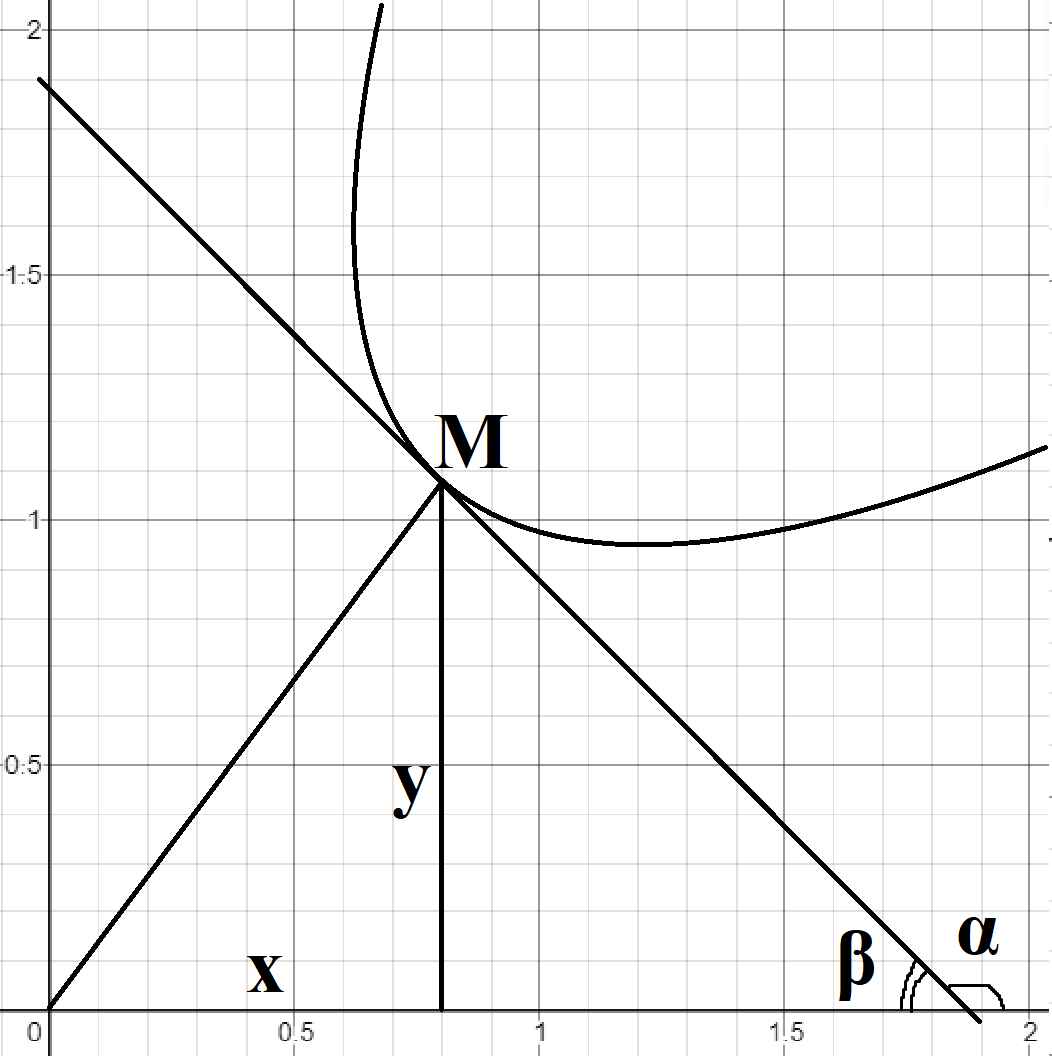
\includegraphics[scale=0.2]{pics/resh6.png}
	    \centering
	\end{figure}
  \[\tg \beta = - \tg \alpha = -y'\]
  \[\frac{1}{2} (x-\frac{y}{y'})y=a^2\]
  \[x y - 2a^2 = y^2 \frac{dx}{dy}\]
\end{example}

\begin{example}[178, мат. анализ наносит ответный удар]
  Найти то решение дифференциального уравнения
  \[y' sin 2x = 2(y + cos x),\]
  которое остается ограниченным при $x \ra \frac{\pi}{2}$\\
\end{example}

\begin{Sol}
  \[y=C\tg x+\frac{1}{\cos x}\]
  Следует, что
\end{Sol}

\begin{Definition}[Риккати]
  \[y'=a(x)y^2+b(x)y+c(x) \q (1)\]
  В общем случае не интегрируется в квадратурах.
  \[y=y_1(x) \text{ - реш (1) $\Ra$ замена }y=z+y_1\]
  \[z'+y_1'=a(z^2+2zy_1+y_1^2)+b(z+y_1)+c\]
  \[z'+\cancel{y_1'}=a(z^2+2zy_1+y_1^2)+bz+\cancel{ay_1^2+by_1}+c\]
  \[z'=(2ay_1+b)z+az^2\text{ - уравнение Бернулли}\]
\end{Definition}

\begin{example}
  Как подбирать? $y'+y^2=x^2+2$\\
  Попробуем подобрать степень x для y: $a^2 x^{2n}+...=x^2-2x$
  \[a=1,\q n=1\]
  \[y=x+c,\q -1+x^2+2xc+c^2=x^2-2x\Ra c=1\]
  \[y=x-1 \Ra -1+x^2-2x+1=x^2-2x\]
\end{example}

\begin{Example}[ещё пример]
  \[y'+2y^2=\frac{6}{x^2}\]
  \[y=\frac{a}{x} \Ra -\frac{a}{x^2}+\frac{2a^2}{x^2}=\frac{6}{x^2}\]
  \[2a^2-a-6=0 \Ra a=2\]
\end{Example}

\begin{Example}[171]
  \[y'+2y e^x - y^2 = e^{2x}+e^x\]
  \[y=e^x+z \Ra z'=z^2 \Ra \frac{dz}{dx}=z^2 \os{z \neq 0}{\Ra} z=-\frac{1}{x+C}\]
  Но при $z=0$ полуаем решение $y=e^x$\\
  Ответ: $y=e^x-\frac{1}{x+C},\q y=e^x$
\end{Example}

\subsection{Уравнения в полных дифференциалах. Интегрирующий множитель}
\begin{Definition}
  \[M(x,y)dx+N(x,y)dy=0 \text{ - уравнение в полных дифф, если } M,N \in C^1(G)\]
  \[\e u(x,y): du= \ub{\frac{\d u}{\d x}=u'_x}{M} dx + \ub{\frac{\d u}{\d y}=u'_y}{N} dy\]
  \[\frac{\d M}{\d y}=u''_{x y}=u''_{y x}=\frac{\d N}{\d x}\]
\end{Definition}

\begin{example}[187]
  Проверить, что данное уравнение является уравнением в полных дифференциалах, и решить его:
  \[\ub{M}{(2 - 9x y^2)x} dx + \ub{N}{(4y^2 - 6x^3)y} dy = 0\]
  \[M'_y=-18x^2 y \qq N'_x=-19 x^2 y\]
  \[M=u'_x \Ra u = \int (2x-9x^2 y^2) dx +\varphi(y)=x^2-3x^2 y^2 + \varphi(y)\]
  \[u'_y=-6x^3 y + \varphi'(y)=N=4y^3-6x^3 y\]
  \[\varphi'(y)=4y^3 \Ra \varphi(y)=y^4\]
  \[u(x,y)=x^2-3x^3 y^2 + y^4\]
  Ответ: $x^2-3x^3 y^2 +y^4 = c$,\q т.к.$du = 0 \Ra u=c$
\end{example}

Для сравнения:
\[\ub{d(x^2)}{2x dx} - \ub{-3(y^2 \ub{d(yx^3)}{3x^2 dx} + x^3 \ub{d(y^2)}{2y dy})}{9x^2 y^2 dx - 6x^3 y dy} + \ub{d(y^4)}{4 y^3 dy}  = 0\]
Дифференциал произведения $d(x^3 y^2)$

\begin{example}[193]
  Проверить, что данное уравнение является уравнением в полных дифференциалах, и решить его:
  \[\ub{d(x^3)}{3x^2 dx}(1 + \ln y) = \ub{-d(y^2)}{2y dy} - x^3 \ub{d(\ln y)}{\frac{1}{y}dy}\]
\end{example}

\begin{Definition}
  \[M(x,y)dx+N(x,y)dy=0 \text{ - уравнение в полных дифф } (1)\]
  \[\mu=\mu(x,y) \text{ - инт. мн-ль }(1)\text{, если }(\mu M)dx+(\mu N)dy=0 \text{ - ур. в полных лиф.}\]
\end{Definition}

\begin{Example}[195, фокус]
  Решить уравнение, найдя каким-либо способом интегрирующий множитель или сделав замену переменных:
  \[(x^2 + y^2 + x)dx + y dy = 0\]
  \[(x^2+y^2)dx + \ub{\frac{1}{2}d(x^2+y^2)}{x dx+y dy} = 0\]
  \[dx+\frac{1}{2} \frac{d(x^2+y^2)}{x^2+y^2}=0\]
  Значит $\mu = \frac{1}{x^2+y^2}$
  \[dx+\frac{1}{2} d \ln (x^2+y^2)=0\]
  Ответ: $x+\frac{1}{2} \ln(x^2+y^2)=c$
\end{Example}

\begin{Example}[196, фокус]
  Решить уравнение, найдя каким-либо способом интегрирующий множитель или сделав замену переменных:
  \[(x^2 + y^2 + x)dx - x dy = 0\]
  \[(x^2+y^2)dx + y dx - x dy = 0\q d \Br{\frac{y}{x}}=\frac{dy x - y dx}{x^2}\]
  \[(1+\Br{\frac{y}{x}}^2)dx - \ub{d\Br{\frac{y}{x}}}{\frac{x dy-y dx}{x^2}}\]
  \[\mu = \frac{1}{x^2(1+\Br{\frac{y}{x}}^2)}=\frac{1}{x^2+y^2}\]
\end{Example}


ДЗ: 167-170 (интересные), 188-194 (интересные), 196, 201, 203

\section{ПРОПУЩЕННАЯ ПАРА}

\section{В ожидании кр...}

\begin{Example}
  \[xy^2(xy'+y) = 1\qq \text{Заметим, что }xy'+y = (xy)'\]
  \[xy'+y-\dfrac{1}{xy^2} = 0 \qq xy = z \Ra \dfrac{z^2}{x}z' = 1\]
  \[x dy + \dfrac{xy^3 - 1}{xy^2}dx = 0\]
  \[x^2 y^2 dy + xy^3 dx - dx = 0\]
  \[\mu = ?\]
  \[\ub{d(xy)}{x dy + y dx} - \dfrac{dx}{xy^2} = 0\]
  \[c = \dfrac{xy^3}{3} + \dfrac{x^2}{2}\]
\end{Example}

\begin{Example}[203]
  \[y(x+y)dx + (xy+1)dy = 0\]
  \[yx dx + y^2 dx + xy dy + dy = 0\]
  \[yx dx + y(\ub{d(xy)}{y dx + x dy}) + dy = 0 | \cdot \dfrac{1}{y}\]
  \[x dx + d(xy) + \dfrac{dy}{y} = 0\]
  \[\dfrac{x^2}{2} + xy + \ln |y| + c = 0\]
\end{Example}

\begin{Example}[301]
  \[xy' + x^2 + xy - y\]
\end{Example}

\begin{Proof}[похоже на частного, на однородное не тянет, но замена проходит]
  \[\dfrac{xy' - y}{x^2} + 1 \dfrac{y}{x} = 0\]
  \[y' = \dfrac{y}{x} + \dfrac{y^2}{x^2}\]
\end{Proof}

\begin{Example}[308]
  \[x^2 y' = y(x+y)\]
\end{Example}

\begin{Proof}[однородное/Бернулли]
  \[y' = \dfrac{x}{y} + \dfrac{y^2}{x^2}\]
\end{Proof}

\begin{Example}[309]
  \[(1-x^2)dy + xy dx\]
\end{Example}

\begin{Proof}[уравнение с разделяющимися переменными]

\end{Proof}

\begin{Example}[311]
  \[(y + y' \ln^2 y = (x+2\ln y)y'\]
\end{Example}

\begin{Proof}[линейное уравнение]
  \[y'_x = \dfrac{1}{x'_y}\]
  \[x'_y y = x + 2\ln y 0 \ln^2 y\]
  \[y dx - x dy (2\ln y - \ln^2 y) dy\]
\end{Proof}

\begin{Example}[320]
  \[2x^3 y y' + 3x^2 y^2 + 7 = 0\]
\end{Example}

\begin{Proof}[производная произведения]
  \[(x^3 y^2)' + 7 = 0'\]
\end{Proof}

\begin{Example}[330]
  \[(1-x^2)y^2 - 2xy^2 = xy\]
\end{Example}

\begin{Proof}[переменные разделяются, Бернелли]

\end{Proof}

\begin{Example}[333]
  \[(\sin x + y) dy + (y \cos x - x^2) dx = 0\]
\end{Example}

\begin{Proof}[уравнение в полных дифференциалах]
  \[\ub{d(y \sin x)}{\sin x dy + y \cos x dx} - y dy - x^2 dx = 0\]
\end{Proof}

\begin{Example}[338]
  \[x(x+1)(y'-1) = y\]
\end{Example}

\begin{Example}[349]
  \[xy' = 2 \sqrt y \cos x - 2y\]
\end{Example}

\begin{Proof}[Бернулли, вариация переменной]

\end{Proof}

\begin{Example}[359]
  \[xy'(\ln y - \ln x) = y\]
\end{Example}

\begin{Proof}[однородное]
  \[y' \ln \dfrac{y}{x} = \dfrac{y}{x}\]
\end{Proof}

\begin{Example}[361]
  \[(2x^2 y - 3y^2)y' = 6x^2 - 2xy^2 +1\]
\end{Example}

\begin{Example}[368]
  \[y' = \sqrt[3]{2x - y} + 2\]
\end{Example}

\begin{Example}[371]
  \[2(x^2 y + \sqrt{1 + x^4 y^2}) dx + x^3 dy\]
\end{Example}

\begin{Example}[374]
  \[(2x+3y-1)dx + (4x + 6y - 5)dy = 0\]
\end{Example}

\begin{Proof}[параллельные прямые]
  \[2x + 3y - 1 = z \Ra 2dx + 3dy = dz\]
\end{Proof}

\begin{Example}[414]
  \[(x^2-1)y' + y^2 - 2xy + 1 = 0\]
\end{Example}

\begin{Example}[438]
  \[(2x + y + 5)y' = 3x + 6\]
\end{Example}

\begin{Proof}[пересекающиеся прямые]
  \[(2x+y+5)dy - (3x+6)dx = 0\]
  \[\text{Замена } x + 2 = \w{x}\q y + 1 = \w{y}\]
\end{Proof}

\section{Уравнения первого порядка, не разрешенные относительно производной}
Если можно разрешить, то разрешим.

\begin{Task}[1]
    \[(y')^2 = 1 \qq \bigg[ \begin{matrix}
        y' = 1\\
        y' = -1
    \end{matrix} \qq \bigg[ \begin{matrix}
        y = x + c\\
        y = -x + c
    \end{matrix}\]
    Если исх. ур. распалось на неск. реш. с ед., то и про исх. говорят, что оно ед.
\end{Task}

\begin{Task}[2]
    \[\sin(y' - 1) = 0\]
    \[y' - 1 = \pi k, \q k \in \Z\]
\end{Task}

\begin{Definition}[Метод введения параметра]
    \[f(x, y, y') = 0\]
    \begin{enumerate}
        \item Разрешить отн $x$ либо отн $y$
            \[y = g(x, y') \qq x = h(y, y')\]
            \[p = y' = \frac{dy}{dx} \text{ - параметр}\]
        \item подставляем
            \[y = g(x, p) \qq x = h(y, p)\]
        \item дифф-уем
            \[pdx = dy = dg(x, p) \qq \frac{dy}{p} = dx = dh(y, p)\]
    \end{enumerate}
    \[\text{Ответ: } \begin{cases}
        x =  x(p) \\
        y = g(x(p), p)
    \end{cases} \qq \begin{cases}
        y = y(p)\\
        x = h(y(p), p)
    \end{cases}\]
\end{Definition}

\begin{Example}[267-286]
  \[y'(x-\ln y') = 1\]
  \[x = \ln y' + \dfrac{1}{y'}\]
  \[y' = p \q y' > 0\]
  \[x = \ln p + \dfrac{1}{p}\]
  \[\dfrac{dy}{p} = dx = \dfrac{dp}{p} - \dfrac{dp}{p^2}\]
  \[\int dy = \int (1-\dfrac{1}{p}) dp\]
  \[\begin{cases}
    y = p - \ln |p| + C\\
    x = \ln p + \dfrac{1}{p}
  \end{cases}\]
\end{Example}

\begin{Example}[280]
  \[x^2 (y')^2 = xyy' + 1\]
  \[y = \dfrac{x^2 (y')^2 - 1}{x y'} = xy' - \dfrac{1}{xy'}\]
  \[y' = p\]
  \[y ' [x - \dfrac{1}{xp}\]
  \[dy = x dp p dx - \dfrac{1}{x^2 p^2} (x dp + p dx)\]
  \[p dx = x dp + p dx + \dfrac{1}{x^2 p^2} (x dp + p dx)\q | x^2 p^2\]
  \[0 = x^3 p dp + x dp + p dx\]
  \[p dx = -(x^3 p^2 + x) dp \text{ - уравнение Бернулли}\]
  \[\dfrac{dx}{dp} = -(x^3 p + \dfrac{x}{p})\]
  \[\dfrac{dx}{dp} = - \dfrac{x}{p}\]
  \[\int \dfrac{dp}{x} = - \int \dfrac{dp}{p} \Ra \ln |x| = \ln |\dfrac{1}{p}| + \ln|C|\]
  \[x \neq 0 \q p \neq 0\]
  \[x = \dfrac{C(p)}{p}\]
  \[\dfrac{C'p - C}{p^2} = \dfrac{-C^3}{p^2} - \dfrac{C}{p^2} \Ra C'p = - C^3\]
  \[\dfrac{dc}{dp} p = - c^3 \Ra \int \dfrac{dc}{c^3} = - \int \dfrac{dp}{p}\]
  \[\dfrac{C^{-2}}{2} = \ln|p| + C^* \Ra \dfrac{1}{C^2} = 2 \ln|p| + C^{**}\]
  \[C = \pm (\sqrt{2 \ln|p| + C^{**}})^{-1} \]
  \[\begin{cases}
    x = \pm \dfrac{1}{p\sqrt{2 \ln|p| + C^{**}}}\\
    y = \pm \dfrac{1}{\sqrt 2 <...>} + \dfrac{1}{p \sqrt{<...>}}
  \end{cases}\]
\end{Example}

%\begin{Example}
  %\[y = y' x + \varphi(y') \text{ - ур. Клеро}\]
  %Всегда касается решения?
 % \[y = f(y')x + g(y') \text{ - ур. Лагранжа}\]
  %%Всегда имеет вид линейного уравнения
%\end{Example}

\begin{Definition}
    \[y = y' x + \varphi(y') \text{ - ур. Клеро}\]
    \[y = f(y')x + g(y') \text{ - ур. Лагранжа}\]
    Уравнение Клеро имеет общ. решение - серию лин. функций (прямые) и особое решение, график которого - 
    огибающаяя сем-ва кривых\\
    Особое рещение - в каждой точке которого много решений (наруш. ед.)\\
    В уравнении Лагранжа мы получаем лин. по $x$ ур. В качестве общ решения мы получим сем-во прямых
\end{Definition}

\begin{Task}[287]
  \[y = xy' - (y')^2\]
  \[y' = p \q dy = p dx\]
  \[y = xp - p^2\]
  \[\cancel{p dx} = \cancel{p dx} + x dp - 2 p dp \text{ (всегда сокращается)}\]
  \[0 = dp(x - 2p)\]
  \begin{enumerate}
    \item $dp = 0 \Ra p = C \Ra y = Cx - C^2$ - общее решение
    \item $x = 2p \Ra y = 2p^2 - p^2 = p^2 \Ra \begin{cases}
      x = 2p\\
      y=p^2
    \end{cases} \q y = \dfrac{x^2}{4}$ - особое решение
  \end{enumerate}
  \begin{figure}[H]
    \centering
    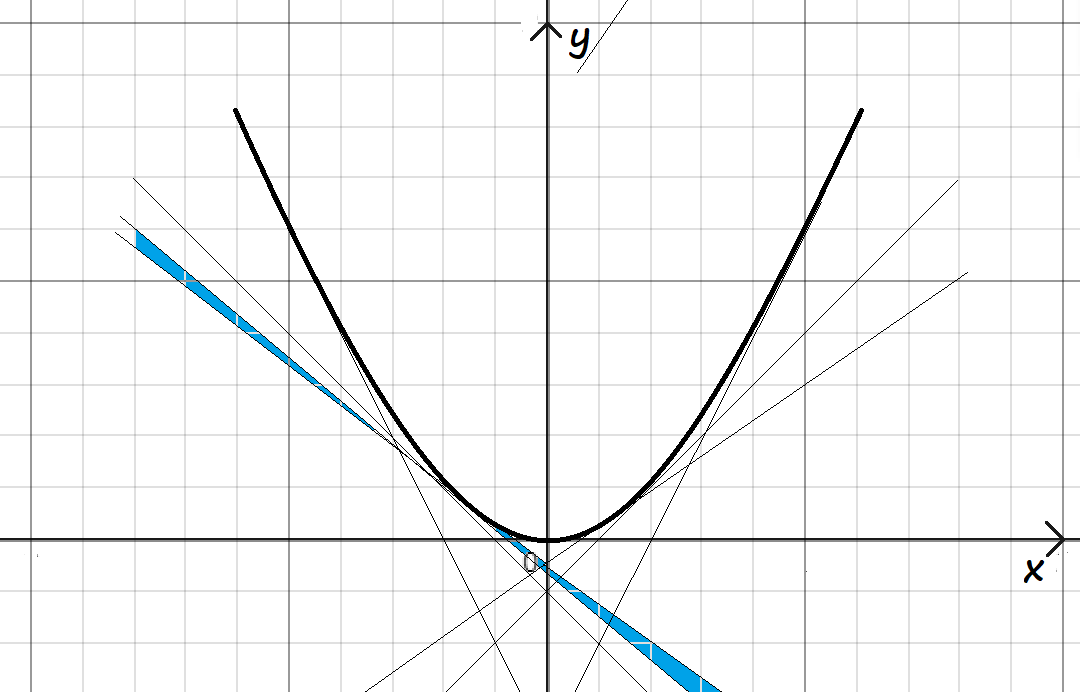
\includegraphics[width=8cm]{parabola}
    \caption*{Прямые образуют параболу}
  \end{figure}
  Через каждую точку параболы проходит бесконечно решений
  \[(y')^2 - xy^2 + y = 0\]
  \[y' = \dfrac{x \pm \sqrt{x^2 - 4y}}{2}\]
\end{Task}
Дз: 264 - 267, 282, 269, 271, 289, 290, 292 (Лагранж)

\begin{Example}[292]
  \[y = x (y')^2 - 2(y')^3\]
  \[y' = p \q y = xp^2 - 2p^3\]
  \[p dx = p^2 dx + 2x p dp - 6p^2 dp\]
  \[(p-p^2) dx = (2xp - 6p^2) dp\]
  \[p = 0 \Ra y = 0\]
  \[p = 1 \Ra y = x - 2\]
  \[\dfrac{dx}{dp} = \dfrac{2x}{1-p} - \dfrac{6p}{1-p} \text{ - линейное уравнение}\]
\end{Example}

\begin{lect}
    \section{Уравнения допускающие понижение порядка}
    \begin{Definition}
        \[F(x, y, y', ..., y^{(n)} ) = 0\]
        \begin{enumerate}
            \item $F(x, y^{(k)}, ..., y^{(n)}  ) = 0$
                \[y^{(k)} = z \q \Ra y^{(k + 1)} = z' \qq F(x, z, z', ..., z^{(n - k)}) \]
            \item $F(y, y', ..., y^{(n)} ) = 0$
                \[y \text{ - новая нез. перем.}\]
                \[y_x' = p(y) \text{ - новая неизв. функция}\]
                \[y''_{xx} = (y'_x)'_x = p'_x = p'_y \cdot \us{p}{y'_x} = p'_y \cdot p \]
                \[y'''_{xxx} = (y''_xx)'_x = (p'_y \cdot p)'_y \cdot y'_x = (p'' \cdot p + (p')^2)p  \]
            \item $F(x, \lambda y, \lambda y', ..., \lambda y^{(n)} ) = \lambda^{s} 
                F(x, y, y', ..., y^{(n)} )  \qq (\forall  \lambda > 0)$
                Суммарная степень слаг. с $y$ и его произв. одинаковая\\
                замена $y' = yz$
                \[\Ra y'' = \us{yz}{y'} \cdot z + y \cdot z' = y(z^2 + z')\]
                \[y''' = yz(z^2 + z') + y(2zz' + z'') = y(z^3 + 3zz' + z'')\]
            \item $F(\lambda \cdot x, \lambda^{m}y, \lambda^{m - 1}y', ..., 
                \lambda^{m - n}y^{(n)}) = \lambda^s F(x, y, y', ..., y^{(n)} )$
                \[\begin{cases}
                    x = e^t\\
                    y = ze^{mt} 
                \end{cases} \qq t \text{ - нов. нез. перем}\]
                \[z = z(t) \text{ - новая ф-я}\]
        \end{enumerate}
    \end{Definition}

    \begin{Task}[438]
        \[y'' - xy''' + (y''')^3 = 0\]
        \[y'' = z \q \Ra z - xz' + (z')^3 = 0\]
        \[z = xz' - (z')^3 \text{ доделать дома}\]
    \end{Task}

    \begin{Task}[436]
        \[(y'')^2 = (y')^2 + 1\]
        \[y' = p\]
        \[y''= p'p\]
        \[(p'p)^2 = p^2 + 1\]
        \[(p')^2p^2 = p^2 + 1\]
        \[p' = \frac{\pm \sqrt{p^2 + 1}}{p}\]
        \[\frac{dp}{dy} = \frac{\pm \sqrt{p^2 + 1}}{p}\]
        \[\frac{pdp}{\sqrt{p^2 + 1}} = \pm dy\]
        \[\sqrt{p^2 + 1} = \pm y + C_1\]
        \[p^2 + 1 = (C_1 \pm y)^2\]
        \[y' = \pm \sqrt{(C_1 \pm y)^2 - 1}\]
        \[\frac{dy}{\sqrt{(C_1 \pm y)^2 - 1}} = \pm dx \]
        \[\int \frac{dt}{\sqrt{t^2 \pm 1}} = \ln \abs{t + \sqrt{t^2 \pm 1}} + C \]
        \[\ln \abs{y \pm C_1 + \sqrt{(y \pm C_1)^2 - 1}} = \pm x + C_2\]
    \end{Task}

    \begin{Task}[226]
        \[yy'' + 1 = (y')^2\]
        \[y' = p\ \Ra\ y'' = p \cdot p'\]
        \[ypp' = p^2 - 1\]
        \[\frac{pdp}{p^2 - 1} = \frac{dy}{y} \qq p = \pm 1\]
        \[y' = \pm 1\]
        \[y = \pm x + C\]
        \[\frac{1}{2}\ln\abs{p^2 - 1} = \ln\abs{y} + \ln \abs{C_1}\]
        \[p^2 - 1 = C_1y^2\]
        \[(y')^2 = C_1y^2 + 1\]
        \[y' = \pm \sqrt{C_1 y^2 + 1}\]
        \[\frac{dy}{\sqrt{c_1y^2 + 1}} = \pm dx\]
        \[C_1 > 0 \qq \frac{1}{\sqrt{C_1}} \int \frac{\sqrt{C_1}dy}{\sqrt{(\sqrt{C_1}y)^2 + 1}}\]
        \[C_1 < 0 \qq \frac{1}{\sqrt{-C_1}} \int \frac{\sqrt{-C_1}dy}{\sqrt{-(\sqrt{-C_1}y)^2 + 1}}\]
        \[C_1 = 0 \qq y = \pm x + C\]
    \end{Task}

    \begin{Task}[?]
        \[xyy'' - x(y')^2 = yy'\]
        \[x(yy'' - (y')^2) = yy'\]
        \[\left(\frac{y'}{y}\right)' = \frac{y'' \cdot y - y' \cdot y'}{y^2}\]
        \[x\frac{yy'' - (y')^2}{y^2} = \frac{y'}{y}\]
        \[\frac{y'}{y} = z \Ra xz' = z\]
    \end{Task}

    \begin{Task}[366]
        \[xyy'' + x(y')^2 = 2yy'\]
        \[x(y \cdot y'' + (y')^2) = 2yy'\]
        \[x\left(y \cdot y'\right)' = 2yy' \qq yy' = z\]
        \[xz' = 2z\]
    \end{Task}

     
    \begin{Task}[466]
        Способ: догадайся
        \[y' \cdot y''' = 2(y'')^2\]
        \[\frac{y'''}{y''} = 2 \frac{y''}{y'} \qq y'' = 0 \Ra y' = C_1 \Ra y = C_1x + C_2\]
        \[(\ln \abs{y})' = \frac{y'}{y}\]
        \[(\ln \abs{y''})' = 2(\ln \abs{y'})'\]
        \[\ln \abs{y''} = 2\ln \abs{y'} + \ln \abs{C_1}\]
        \[y'' = C_1 (y')^2\]
        \[\frac{y''}{y'} = C_1 y'\]
        \[(\ln \abs{y'})' = C_1 y'\]
        \[\ln \abs{y'} = C_1 y + \ln \abs{C_2}\]
        \[y' = C_2 \cdot e^{C_1 y} \]
    \end{Task}

    \begin{Task}[?]
        \[x^3 y'' = (y - xy')(y - xy' - x)\]
        \[x^3 y'' = y^2 - 2xyy' + x^2(y')^2 - xy + x^2 y'\]
        \[3 + m - 2 = 2m = 1 + m + m -1 = 2 + 2(m - 1) = 1 + m = 2 + m - 1\]
        \[m + 1 = 2m = ... = m + 1 = ...\]
        \[\Ra m = 1\]
        \[y = ze^{mt} \qq x = e^t \]
        \[y'_x = \frac{y'_t}{x'_t} = \frac{z' e^{mt} + zm e^{mt}  }{e^t} = (z' + mz)e^{(m - 1)t} \]
        \[y''_{xx} = (...) e^{(m - 2)t}  \]
        доделать дома
    \end{Task}

    ДЗ: \ 421-450, 449, 442, 467, 469\\
    462 "догадайся"
    

\end{lect}

\begin{lect}
    \section{линейные уравнения n-ого порядка}
    \begin{Definition}
    \[L(y) = y^{(n)} + p_1(x)y^{(n - 1)} + ... + p_{n - 1}(x)y' + p_n(x)y   \]
    \[(1) \q L(y) = 0 \q \text{ л.о.у}\]
    \[(2) \q L(y) = q(x) \q (q(x) \not \equiv 0) \q \text{ л.н.у}\]
    \[p_i(x), q(x) \in C(a, b)\]
    \[\Ra  \forall \text{ З.К } \q (x_0, y_0, y_0', ..., y_0^{(n - 1)} ) \]
    имеет ед. решение, продолжимое на $(a, b)$, если $x_0 \in (a, b)$
    \\
    Рассмотрим (1) $\exists $ фунд. система решений $\varphi_1(x), ..., \varphi_n(x)$ - n лин. нез. решений
    \[\Ra y_{\text{общ однор}}(x) = c_1 \varphi_1(x) + ... + c_n \varphi_n(x) \qq (3) \qq c_j = const \]

    \[(1') \q y^{(n)} + a_1 y^{(n - 1)} + ... + a_{n - 1}y' + a_n y = 0 \]
    \[y = e^{\lambda x} \text{ - реш } (1') \rla
        \underbracket{\lambda^n + a_1 \lambda^{n - 1} + ... + a_{n - 1} \lambda + a_n}_{\text{хар мн-н 
    $P(\lambda)$}}  = 0 \qq (4)\]
    \[(4) \text{ - характ. ур-е}\]
    \[\text{корни } \lambda_1, ..., \lambda_n \text{ - хар. числа}\]
    \begin{enumerate}
        \item $\lambda_1, ..., \lambda_n$ - вещ, различные $\Ra e^{\lambda_1x}, ..., e^{\lambda_n x}$ - ф.с.р
        \item $\lambda_j = \alpha + i\beta $ - корень (простой кратности. 1) хар. ур. $\Ra \overline{\lambda}_j
            = \alpha - i\beta$ - тоже..
            \[e^{\lambda_jx} = e^{\alpha x} \q (\cos \beta x + i\sin \beta x)\]
            Решения в ф.с.р. отв-е $\lambda_j, \overline{\lambda}_j$
            \[e^{\alpha x} \cos \beta x  \]
            \[e^{\alpha x} \sin \beta x  \]
        \item $\lambda_j$ - вещ, кратности $d \geq 2 \to  e^{\lambda_jx}, xe^{\lambda_j x}, ..., 
            x^{d - 1}e^{\lambda_j x}   $
        \item $\lambda_j = \alpha + i \beta $ - корень $(4)$ кр. $d \geq 2 \Ra \overline{\lambda}_j$ - тоже... 
            \[(\beta \neq 0)\]
            \[2d \text{ реш } \q \begin{matrix}
                e^{\alpha x} \cos \beta x, x e ^{\alpha x} \cos \beta x, ...., x^{d - 1} e^{\alpha x}
                \cos \beta x\\
                 e^{\alpha x} \sin \beta x, x e ^{\alpha x} \sin \beta x, ...., x^{d - 1} e^{\alpha x}
                \sin \beta x
            \end{matrix}\]
    \end{enumerate}
    \end{Definition}

    \begin{Task}[529]
        \[y^{(4)} - 5y'' + 4y = 0 \]
        \[\lambda^4 - 5 \lambda^2 + 4 = 0\]
        \[\lambda = \pm 2,\ \pm 1\]
        \[y_{\text{оо}}  = C_1 e^{2x} + C_2 e^{-2x} + C_3 e^{x} + C_4 e^{-x}    \]
    \end{Task}

    \begin{Task}[530]
        \[y^{(5)} + 8y'''  +16y' = 0 \]
        \[\lambda^5 + 8\lambda^3 + 16\lambda = 0\]
        \[\lambda = 0\]
        \[\lambda = \pm 2i \text{ кр } 2\]
        \[y = C_1 + C_2 \cos(2x) + C_3 \sin(2x) + C_4 x \cos(2x) + C_5 x \sin(2x)\]
    \end{Task}

    \begin{Task}[531]
        \[y''' - 3y' + 2y = 0\]
        \[\lambda^3 - 3\lambda + 2 = 0\]
        \[\lambda = 1 \text{ - кр } 2\]
        \[\lambda = -2\]
        \[y = C_1 e^x + C_2 x e^x + C_3 e^x\]
    \end{Task}

    \begin{Task}[532]
        \[y^{(4)} + 4y'' + 3y = 0 \]
        \[\lambda^4 + 4\lambda^2 + 3 = 0\]
        \[\lambda = \pm i \sqrt{3}\]
        \[\lambda \pm i\]
        \[y = C_1 \cos (\sqrt{3}x) + C_2 \sin(\sqrt{3}x)  +C_3 \cos x + C_4 \sin x\]
    \end{Task}

    \begin{Definition}
        \[(2) \q L(y) = q(x)\]
        \[y_{\text{общ неоднор}}  = y_{\text{общ однор}} + \psi_{\text{частн неоднор}}   \]
        \[(y_{\text{он}} = y_{\text{оо}} + \psi_{\text{чн}}   )\]
        \begin{enumerate}
            \item Метод вариации произвольных постоянных
            \item Метод неопред. коэф.
        \end{enumerate}
        Метод неопред. коэф. не требует интегрирования
    \end{Definition}

    \begin{Remark}
        \[\text{в } (2) \q q = q_1 + q_2\]
        \[\psi_1 \text{ - реш ур } L(y) = q_1\]
        \[\psi_2 \text{ - реш ур } L(y) = q_2 \]
        \[\Ra L(\psi_1 + \psi_2) = L(\psi_1) + L(\psi_2) = q\]
        \[\Ra (\psi_1 + \psi_2) \text{ - реш } (2)\]
    \end{Remark}

    \begin{Definition} [Метод неопред коэф.]
        \[\RNumb{1}\]
        \[q(x) = e^{\lambda x} \us{\text{мн-н ст m}}{ P_m(x)} \]
        \[\Ra (2) \text{ имеет решение вида } \psi(x) = x^s \cdot e^{\lambda x} \cdot
        \us{\text{мн-н ст m}}{ Q_m(x)} \]
        \[s = 0, \text{ если } \lambda \text{ - не корень } (4)\]
        В противном случае $s$ - кратность $\lambda$ как корня хар. ур $(4)$ (ур $(1')$)
        \[\RNumb{2}\]
        \[q(x) = e^{\alpha x} (\widetilde{P_{m_1} }(x) \cos \beta x + \widetilde{\widetilde{P}}_{m_2}  
        (x)\sin \beta x) \]
        \[\Ra (2) \text{ имеет реш. вида } \psi(x) = x^se^{\alpha x} (\widetilde{Q}_m(x)\cos \beta x + 
        \widetilde{\widetilde{Q}}_m(x)\sin \beta x)\]
        \[m = \max(m_1, m_2), \q s = 0, \text{ если } \lambda = \alpha + i\beta \text{ - не корень } (4)\]
        В противном случае $s$ - кратность $\lambda$ как корня хар. ур $(4)$
    \end{Definition}

    \begin{Task}
        \[y'' + 6y' + 10y = 3x^2e^{3x} - 2xe^{-3x} \cos x + sh(3x)  \]
        \[\lambda^2 + 6\lambda + 10 = 0\]
        \[\lambda = -3 \pm i\]
        \[y_{\text{оо}} = e^{-3x} (C_1 \cos x + C_2 \sin x) \]
        \[sh(3x) = \frac{e^{3x} - e^{-3x}  }{2}\]
        \[y'' + 6y' + 10y = \us{q1}{(3x^2 + \frac{1}{2})e^{3x}} -\us{q2}{ 2xe^{-3x} \cos x} - 
        \us{q3}{\frac{1}{2}e^{-3x}}   \]
        \[1)\q L(y) = q_1 \qq \psi_1(x) = e^{3x}(a_1 x^2 + b_1x + c_1) \]
        \[2)\q L(y) = q_2 \qq \psi_2(x) = x^{-3x}(a_2x + b_2)\cos x + (a_3x + b_3)\sin x \]
        \[3)\q L(y) = q_3 \qq \psi_3(x) = a_4 e^{-3x} \]
    \end{Task}


    \begin{Definition}
        \[\ddot{x} + k^2x = 0 \text{ - уравнение свободных колебаний}\]
        \[\lambda^2 + k^2 = 0 \qq \lambda \pm ik\]
        \[x_{\text{оо}}(t) = C_1 \cos kt + C_2 \sin kt \]
        \[\ddot{x} + k^2x = A \sin wt\]
        \[w \neq \pm k \Ra x(t) = x_{\text{оо}}(t) + \underbracket{a_1\cos wt + b_1 \sin wt}_{x_{\text{чн}} }  \]
        \[w = \pm k \Ra x(t) = x_{\text{оо}}(t) + t(a_1 \cos wt + b_1 \sin wt)\]
    \end{Definition}
   % \begin{remark}
    %    Если $s \neq 0$, то говорят, что в уравнении резонанс
    %\end{remark}
    \begin{Task}
        \[y'' + 6y' + 10y = 3x e^{3x} \]
        \[\psi(x) = e^{3x}(ax + b) \]
        \[\psi'(x) = e^{3x}(3ax + 3b + a) \]
        \[\psi''(x) = e^{3x}(9ax + 9b + 6a) \]
        \[(9ax + 9b + 6a) + 6(3ax + 3b + a) + 10(ax + b) = 3x\]
        \[\begin{cases}
            37a = 3
            37b + 12a = 0
        \end{cases}\]
        \[a = \frac{3}{37}\]
        \[b = - \frac{36}{(37)^2}\]
        \[y_{\text{он}} = y_{\text{оо}} + e^{3x}\left(\frac{3}{37}x - \frac{36}{37^2}\right) \]
    \end{Task}

    Дз: 543, 548 (доделать), 569-574 (любой), 564, 573, 566, 570, 582, 584, 586
\end{lect}


\begin{lect}{2019-11-28}
    \begin{Definition}
        пропуск
        \[\begin{cases}
            
        \end{cases}\]
    \end{Definition}
    \begin{Task}
        \[y'' + 4y = 2\tg x\]
        \[\lambda^2 + 4 = 0 \qq \lambda = \pm 2i\]
        \[y_{\text{оо}}(x) = C_1 \sin 2x + C_2 \cos 2x\]
        \[\begin{cases}
            C_1'\sin 2x + C_2' \cos 2x = 0\\
            2C'_1 \cos 2x - 2C_2'\sin 2x= 2 \tg x
        \end{cases}\]
        \[C'_1 = \tg x \cos 2x = \frac{\sin x}{\cos x} (2\cos^2 x - 1)\]
        \[C'_2 = -\tg x \sin 2x = - \frac{\sin x}{\cos x} 2\sin x \cos x = -2\sin^2 x = \cos 2x - 1\]
        \[C_1 = \int \frac{\sin x}{\cos x}(2\cos^2 x - 1)dx \us{u = \cos x}{=} 
        -\int \frac{2u^2 - 1}{u}du = -\int (2u - \frac{1}{u})du\]
        \[= -\cos^2 x + \ln \abs{\cos x} + \widetilde{C}_1\]
        \[C_2 = \int (\cos 2x - 1)dx = \frac{\sin 2x}{2} - x + \widetilde{C}_2\]
        \[y_{\text{он}}(x) = (- \cos^2 x + \ln \abs{\cos x} + \widetilde{C}_1)\sin 2x + 
        \left(\frac{\sin 2x}{2} - x + \widetilde{c}_2\right)\cos 2x\]
        \[y_{\text{он}}(x) = \widetilde{C}_1\sin 2x + \widetilde{C}_2 \cos 2x + (-\cos^2 x \sin 2x +  \]
        \[+ \ln \abs{\cos x}\sin 2x + \frac{1}{2}\sin 2x\cos 2x - x\cos 2x)\]
        \[=\widetilde{C}_1\sin 2x + \widetilde{C}_2 \cos 2x + \left(-\frac{1}{2}\sin 2x + 
        \ln \abs{\cos x}\sin 2x - x\cos 2x\right)\]
    \end{Task}

    \subsection{Уравнение Эйлера}

    \begin{Definition}
        \[a_0 x^{n}y^{(n)} + a_1 x^{n - 1}y^{(n - 1)} + ... + a_{n - 2}x^2 y'' + a_{n - 1}xy' + a_ny = 0\]
        \[x = e^t \text{, если } x > 0 \q (x = -e^t \text{, если $x < 0$})\]
        Замена приводит к уравнению с пост. коэф.
        \[xy'_x = e^t \frac{y'_t}{x'_y} = y'_t \qq y'_x = y'_t e^t\]
        \[x^2y''_{xx} = e^{2t} (y'_x)'_x = e^{2t} \frac{(y'_x)'_t}{x'_t} = e^{2t} 
        \frac{y''_{tt}e^{-t} - y'_te^{-t}   }{e^t} y''_{tt} - y'_t    \]
        \[x^3y'''_{xxx} \to \lambda(\lambda - 1)(\lambda - 2) \]
        \[x^ky_x^{(k)} \to \lambda(\lambda - 1)(\lambda -  2) ... (\lambda - k + 1) \]
    \end{Definition}

    \begin{Task}[2]
        \[x^3y''' - x^2y'' + 2xy' - 2y = x^3 \qq x = e^t\]
        \[\lambda(\lambda - 1)(\lambda - 2) - \lambda(\lambda - 1) + 2\lambda - 2 = 0\]
        \[(\lambda - 1)(\lambda^2 - 3\lambda + 2) = 0\]
        \[(\lambda - 1)^2(\lambda - 2) = 0\]
        \[\lambda = 1 \text{ кр 2}\]
        \[\lambda = 2\]
        \[\Ra y_{\text{оо}}(t) = C_1e^t + C_2 te^t + C_3 e^{2t}  \]
        \[y_{\text{оо}}(x) = C_1 x + C_2 x \ln \abs{x} + C_3 x^2 \]
        \[\lambda^3 -4\lambda^2 + 5\lambda - 2 = 0\]
        \[y'''_{t}  - 4y''_{t} + 5y' -  2y =  e^{3t} \]
        \[y_{\text{чн}}(t) = ae^{3t}  \]
        \[y' = 3ae^{3t} \]
        \[y'' = 9ae^{3t} \]
        \[y'''= 27ae^{3t} \]
        \[27a - 4 \cdot 9 a + 5 \cdot 3 a - 2a = 1\]
        \[a = \frac{1}{4}\]
        \[y_{\text{он}}(x) = C_1 x + C_2 x \ln \abs{x} + C_3 x^2 + \frac{1}{4}x^3 \]
    \end{Task}

    \begin{Task}[600]
        \[(2x + 3)^3y''' + 3(2x + 3)y' - 6y = 0\]
        \[2x + 3 = e^t\]
        \[(2x + 3)y'_x = e^t \frac{y'_t}{x'_t} = e^t \frac{y'_t}{\frac{1}{2}e^t} = 2y'_t \]
    \end{Task}

    \begin{Task}[610]
        \[x^2y'' - xy' + y = \frac{\ln x}{x} + \frac{x}{\ln x}\]
        \[x = e^t\]
        \[\lambda(\lambda - 1) - \lambda + 1 = 0\]
        \[(\lambda - 1)^2 = 0\]
        \[\lambda = 1 \text{  кр 2}\]
        \[y_{oo} = C_1e^t + C_2e^tt \]
        \[y_{oo} = C_1x + C_2 x\ln x \]
        \[\lambda^2 - 2\lambda + 1 = 0\]
        \[y''_t - 2y'_t + y = \frac{t}{e^t} + \frac{e^t}{t}\]
        \[y''_t - 2y'_t + y = te^{-t} + e^t (t^{-1} ) \]
        \[y = (at + b)e^{-t} \]
        \[y' = (a - at - b)e^{-t} \]
        \[y'' = (-a - a + at + b)e^{-t} \]
        \[-2a + at + b - 2a + 2a + 2b + at + b = t\]
        \[(2x + a + x) = -1 \q a = \frac{1}{4}\]
        \[b - 2a - 2a + 2b + b = 0\]
        \[4b - 1 = 0\]
        \[b = \frac{1}{4}\]
        \[y(t) = \frac{1}{4} (t + 1)e^{-t} \]
        \[y_1(x) = \frac{1}{4} \frac{(\ln x + 1)}{x}\]
        \[\]
    \end{Task}

    \begin{Task}[из дз]
        \[y^2(y'\cdot y''' - (y'')^2) - 2(y')^2 (yy'' - (y')^2) + \frac{yy'}{x} (yy'' - 2(y')^2) = 0\]
        \[x \frac{y'y''' - (y'')^2}{(y')^2} - 2x \frac{yy'' - (y')^2}{y^2} + \frac{yy'' - 2(y')^2}{yy'} = 0\]
        \[x \left(\left(\frac{y''}{y''}\right)' - 2 \left(\frac{y'}{y}\right)'\right) + 
        \left(\frac{y''}{y'} - 2\frac{y'}{y}\right) = 0\]
        \[xz' + z = 0 \qq (xz)' = 0\]
    \end{Task}

    \begin{Task}[из дз]
        \[x^2(yy''' - y'y'') = 2yy' - 2x(y')^2\]
        \[x^2 \frac{yy''' - y'y''}{y^2} = \frac{2 y'(y - xy')}{y^2} \qq \left(\frac{y'}{y}\right)' = 
        \frac{y''y - (y')^2}{y^2} \Ra \frac{y''}{y} = \left(\frac{y'}{y}\right)' + \frac{(y')^2}{y^2}\]
        \[x^2 \left(\frac{y''}{y}\right)' + 2x \left(\frac{y''}{y}\right) = 
        \frac{2y'}{y} - 2x \frac{(y')^2}{y^2} + 2x \left(\left(\frac{y'}{y}\right)' + \frac{(y')^2}{y^2}\right)\]
    \end{Task}
\end{lect}

\end{document}
